\documentclass[11pt]{article}
\usepackage{amsgen,amsmath,amstext,amsbsy,amsopn,amssymb}
%\usepackage[dvips]{graphicx,color}
\usepackage{graphicx,color}
\usepackage{graphicx,color,bm}
\usepackage{epsfig}
\usepackage{enumerate}
\usepackage{float}

%\setlength{\oddsidemargin}{0.1 in} \setlength{\evensidemargin}{-0.1
%in} \setlength{\topmargin}{-0.6 in} \setlength{\textwidth}{6.5 in}
%\setlength{\textheight}{8.5 in} \setlength{\headsep}{0.75 in}
%\setlength{\parindent}{0 in} \setlength{\parskip}{0.1 in}

\textwidth 6.3in \textheight 8.8in \topmargin -0.5truein
\oddsidemargin .15truein
\parskip .1in
\renewcommand{\baselinestretch}{1.53}  % double spaced


\newcommand{\homework}[9]{
	\pagestyle{myheadings}
	\thispagestyle{plain}
	\newpage
	\setcounter{page}{1}
	\noindent
	\begin{center}
		\framebox{
			\vbox{\vspace{2mm}
				\hbox to 6.28in { {\bf Math531:~Regression - I  \hfill} }
				\vspace{6mm}
				\hbox to 6.28in { {\Large \hfill #1 (#2)  \hfill} }
				\vspace{6mm}
				\hbox to 6.28in { {\it Instructor: #3 \hfill} }
				\hbox to 6.28in { {\it Office hours: #4  \hfill #6}}
				\vspace{2mm}}
		}
	\end{center}
	\markboth{#1}{#1}
	\vspace*{4mm}
}

% ----------------------- MATH -------------------------
\def\av{\boldsymbol a}
\def\bv{\boldsymbol b}
\def\cv{\boldsymbol c}
\def\dv{\boldsymbol d}
\def\ev{\boldsymbol e}
\def\fv{\boldsymbol f}
\def\gv{\boldsymbol g}
\def\hv{\boldsymbol h}
\def\iv{\boldsymbol i}
\def\gv{\boldsymbol j}
\def\kv{\boldsymbol k}
\def\lv{\boldsymbol l}
\def\mv{\boldsymbol m}
\def\nv{\boldsymbol n}
\def\ov{\boldsymbol o}
\def\pv{\boldsymbol p}
\def\qv{\boldsymbol q}
\def\rv{\boldsymbol r}
\def\sv{\boldsymbol s}
\def\tv{\boldsymbol t}
\def\uv{\boldsymbol u}
\def\vv{\boldsymbol v}
\def\wv{\boldsymbol w}
\def\xv{\boldsymbol x}
\def\yv{\boldsymbol y}
\def\zv{\boldsymbol z}
\def\Av{\boldsymbol A}
\def\Bv{\boldsymbol B}
\def\Cv{\boldsymbol C}
\def\Dv{\boldsymbol D}
\def\Ev{\boldsymbol E}
\def\Fv{\boldsymbol F}
\def\Gv{\boldsymbol G}
\def\Hv{\boldsymbol H}
\def\Iv{\boldsymbol I}
\def\Gv{\boldsymbol J}
\def\Kv{\boldsymbol K}
\def\Lv{\boldsymbol L}
\def\Mv{\boldsymbol M}
\def\Nv{\boldsymbol N}
\def\Ov{\boldsymbol O}
\def\Pv{\boldsymbol P}
\def\Qv{\boldsymbol Q}
\def\Rv{\boldsymbol R}
\def\Sv{\boldsymbol S}
\def\Tv{\boldsymbol T}
\def\Uv{\boldsymbol U}
\def\Vv{\boldsymbol V}
\def\Wv{\boldsymbol W}
\def\Xv{\boldsymbol X}
\def\Yv{\boldsymbol Y}
\def\Zv{\boldsymbol Z}
\def\Abf{\mathbf A}
\def\Bbf{\mathbf B}
\def\Cbf{\mathbf C}
\def\Dbf{\mathbf D}
\def\Ebf{\mathbf E}
\def\Fbf{\mathbf F}
\def\Gbf{\mathbf G}
\def\Hbf{\mathbf H}
\def\Ibf{\mathbf I}
\def\Gbf{\mathbf J}
\def\Kbf{\mathbf K}
\def\Lbf{\mathbf L}
\def\Mbf{\mathbf M}
\def\Nbf{\mathbf N}
\def\Obf{\mathbf O}
\def\Pbf{\mathbf P}
\def\Qbf{\mathbf Q}
\def\Rbf{\mathbf R}
\def\Sbf{\mathbf S}
\def\Tbf{\mathbf T}
\def\Ubf{\mathbf U}
\def\Vbf{\mathbf V}
\def\Wbf{\mathbf W}
\def\Xbf{\mathbf X}
\def\Ybf{\mathbf Y}
\def\Jbf{\mathbf J}
\def\Zbf{\mathbf Z}
\def\Am{\mathrm A}
\def\Bm{\mathrm B}
\def\Cm{\mathrm C}
\def\Dm{\mathrm D}
\def\Em{\mathrm E}
\def\Fm{\mathrm F}
\def\Gm{\mathrm G}
\def\Hm{\mathrm H}
\def\Im{\mathrm I}
\def\Gm{\mathrm J}
\def\Km{\mathrm K}
\def\Lm{\mathrm L}
\def\Mm{\mathrm M}
\def\Nm{\mathrm N}
\def\Om{\mathrm O}
\def\Pm{\mathrm P}
\def\Qm{\mathrm Q}
\def\Rm{\mathrm R}
\def\Sm{\mathrm S}
\def\Tm{\mathrm T}
\def\Um{\mathrm U}
\def\mv{\mathrm V}
\def\Wm{\mathrm W}
\def\Xm{\mathrm X}
\def\Ym{\mathrm Y}
\def\Zm{\mathrm Z}
\newcommand{\Ac}{\mathcal{A}}
\newcommand{\Bc}{\mathcal{B}}
\newcommand{\Cc}{\mathcal{C}}
\newcommand{\Dc}{\mathcal{D}}
\newcommand{\Ec}{\mathcal{E}}
\newcommand{\Fc}{\mathcal{F}}
\newcommand{\Gc}{\mathcal{G}}
\newcommand{\Hc}{\mathcal{H}}
\newcommand{\Ic}{\mathcal{I}}
\newcommand{\Jc}{\mathcal{J}}
\newcommand{\Kc}{\mathcal{K}}
\newcommand{\Lc}{\mathcal{L}}
\newcommand{\Mc}{\mathcal{M}}
\newcommand{\Nc}{\mathcal{N}}
\newcommand{\Oc}{\mathcal{O}}
\newcommand{\Pc}{\mathcal{P}}
\newcommand{\Qc}{\mathcal{Q}}
\newcommand{\Rc}{\mathcal{R}}
\newcommand{\Sc}{\mathcal{S}}
\newcommand{\Tc}{\mathcal{T}}
\newcommand{\Uc}{\mathcal{U}}
\newcommand{\Vc}{\mathcal{V}}
\newcommand{\Wc}{\mathcal{W}}
\newcommand{\Xc}{\mathcal{X}}
\newcommand{\Yc}{\mathcal{Y}}
\newcommand{\Zc}{\mathcal{Z}}
\newcommand{\alphav}{\mbox{\boldmath{$\alpha$}}}
\newcommand{\betav}{\mbox{\boldmath{$\beta$}}}
\newcommand{\gammav}{\mbox{\boldmath{$\gamma$}}}
\newcommand{\deltav}{\mbox{\boldmath{$\delta$}}}
\newcommand{\epsilonv}{\mbox{\boldmath{$\epsilon$}}}
\newcommand{\zetav}{\mbox{\boldmath$\zeta$}}
\newcommand{\etav}{\mbox{\boldmath{$\eta$}}}
\newcommand{\iotav}{\mbox{\boldmath{$\iota$}}}
\newcommand{\kappav}{\mbox{\boldmath{$\kappa$}}}
\newcommand{\lambdav}{\mbox{\boldmath{$\lambda$}}}
\newcommand{\muv}{\mbox{\boldmath{$\mu$}}}
\newcommand{\nuv}{\mbox{\boldmath{$\nu$}}}
\newcommand{\xiv}{\mbox{\boldmath{$\xi$}}}
\newcommand{\omicronv}{\mbox{\boldmath{$\omicron$}}}
\newcommand{\piv}{\mbox{\boldmath{$\pi$}}}
\newcommand{\rhov}{\mbox{\boldmath{$\rho$}}}
\newcommand{\sigmav}{\mbox{\boldmath{$\sigma$}}}
\newcommand{\tauv}{\mbox{\boldmath{$\tau$}}}
\newcommand{\upsilonv}{\mbox{\boldmath{$\upsilon$}}}
\newcommand{\phiv}{\mbox{\boldmath{$\phi$}}}
\newcommand{\varphiv}{\mbox{\boldmath{$\varphi$}}}
\newcommand{\chiv}{\mbox{\boldmath{$\chi$}}}
\newcommand{\psiv}{\mbox{\boldmath{$\psi$}}}
\newcommand{\omegav}{\mbox{\boldmath{$\omega$}}}
\newcommand{\Sigmav}{\mbox{\boldmath{$\Sigma$}}}
\newcommand{\Lambdav}{\mbox{\boldmath{$\Lambda$}}}
\newcommand{\Deltav}{\mbox{\boldmath{$\Delta$}}}
\newcommand{\Omegav}{\mbox{\boldmath{$\Omega$}}}
\newcommand{\varepsilonv}{\mbox{\boldmath{$\varepsilon$}}}

\newcommand{\eps}{\varepsilon}
\newcommand{\epsv}{\mbox{\boldmath{$\varepsilon$}}}

\def\1v{\mathbf 1}
\def\0v{\mathbf 0}
\def\Id{\mathbf I} % identity matrix
\newcommand{\ind}[1]{\mathbbm{1}_{\left[ {#1} \right] }}
\newcommand{\Ind}[1]{\mathbbm{1}_{\left\{ {#1} \right\} }}
\newcommand\indep{\protect\mathpalette{\protect\independenT}{\perp}}\def\independenT#1#2{\mathrel{\rlap{$#1#2$}\mkern2mu{#1#2}}}
\newcommand{\QED}{\begin{flushright} {\bf QED} \end{flushright}}
\newcommand{\R}{\mathbb R}
\newcommand{\Real}{\mathbb R}
\newcommand{\C}{\mathbb C}
\newcommand{\E}{\mathbb E}
\newcommand{\sgn}{\mathop{\mathrm{sign}}}
\def\Pr{\mathrm P}
\def\pr{\mathrm P}
\newcommand{\Var}{\mathop{\rm Var}}
\newcommand{\var}{\mathop{\rm Var}}
\newcommand{\Cov}{\mathop{\rm Cov}}
\newcommand{\cov}{\mathop{\rm Cov}}
\newcommand{\Corr}{\mathop{\rm Corr}}
\newcommand{\ang}{\mathop{\rm Angle}}
\newcommand{\tr}{\mathop{\rm trace}}
\newcommand{\proj}{\mathop{\rm Proj}}
\newcommand{\rank}{\mathop{\rm rank}}

\newcommand{\diag}{\mathop{\rm diag}}
\newcommand{\Diag}{\mathop{\rm diag}}
\newcommand{\sk}{\vspace{0.5cm}}
\newcommand{\ds}{\displaystyle}
\newcommand{\mb}{\mbox}
\newcommand{\wh}{\widehat}
\newcommand{\argmin}{\operatornamewithlimits{argmin}}
\newcommand{\argmax}{\operatornamewithlimits{argmax}}

\newcommand{\norm}[1]{\|#1\|}
\newcommand{\abs}[1]{\left\vert#1\right\vert}
\newcommand{\set}[1]{\left\{#1\right\}}

\newcommand{\To}{\longrightarrow}

\def\equalLaw{\stackrel{\mathcal{L}}{=}}
\def\equallaw{\stackrel{\mathcal{L}}{=}}

\def\half{\frac{1}{2}}

\usepackage{caption}

\begin{document}

\begin{title}
	{\Large\bf Homework 5, DATA 556: Due Tuesday, 10/31/2018}
\end{title}

\author{\bf Alexander Van Roijen}

\maketitle

\newpage
Please complete the following:
\begin{enumerate}
\item Problem 1
Let $U \sim $Unif(a, b).
\begin{enumerate}
	\item Use simulations in R (the statistical programming language) to numerically estimate the median and
	the mode of U for a = 0 and b = 2.
	\begin{verbatim}
	> binUnif= function(n,a,b)
	+ {
	+   resultsog = runif(n,a,b)
	+   results = floor(resultsog*10)
	+   data = data.frame(results)
	+   vals = seq(a,b,.1)
	+   p<-ggplot(data=data, aes(x=factor(data[,1]))) +geom_bar(stat="count") + scale_x_discrete(labels=vals)
	+   p
	+   #barplot(results,main="whatev",width=0.5)
	+   print(median(resultsog))
	+   getmode = table(resultsog)
	+   print(which.max(getmode))
	+   #print(forMode[c(1:10),])
	+ }
	> #this is 1a
	> set.seed(123)
	> n=1000000
	> binUnif(n,0,2)
	[1] 0.9983065
	0.0349205480888486 
	17519 
	\end{verbatim}
	\begin{figure}[H]
		\centering
		\caption{Mode roughly equivalent across all values of x}
		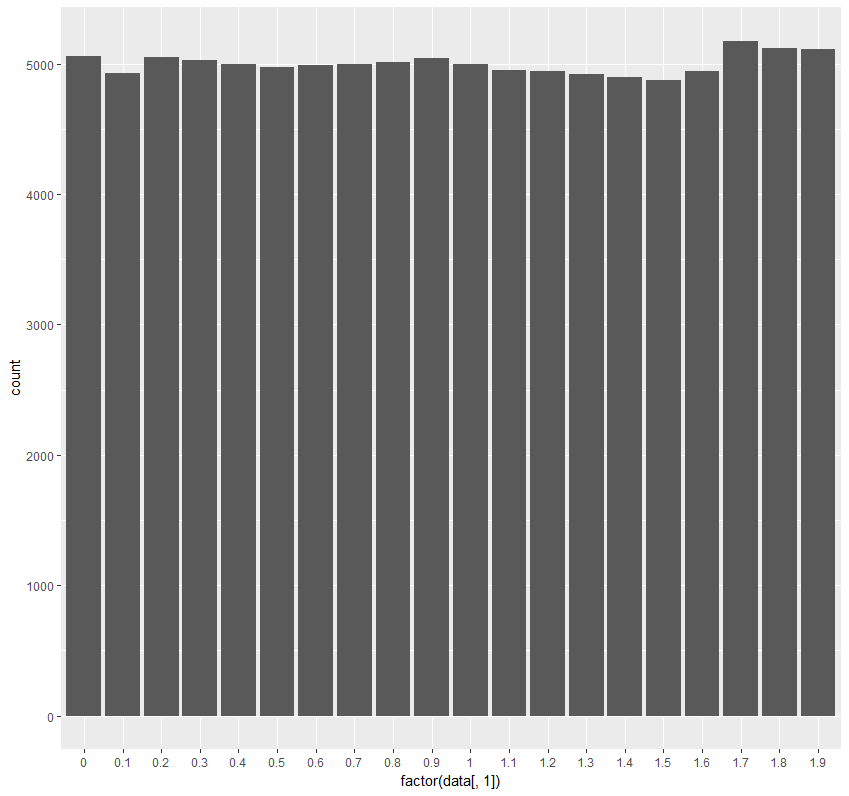
\includegraphics[scale=.6]{Rplot.png}
	\end{figure}
	\item Find the Median and Mode of $U \sim $ Unif(a,b)
	\begin{gather}
	\text{Take the result form above and take the derivative }\\
	f(X|X>a) = F'(X|X>a) = \frac{dF(X|X>a)}{dx} = \frac{F'(x)-F'(a)}{1-F(a)} \text{ with} \frac{dF(a)}{dx} = 0 \\
	=> f(X|X>a) =\frac{f(x)}{1-F(a)}
	\end{gather}
\end{enumerate}
\item Let $ X \sim  $ Expo($ \lambda $)
\\
\begin{enumerate}
	\item Use R to simulate median and mode of Expo(2)
	\\
	\begin{verbatim}
	expoMedMode = function(n,rate)
	+ {
	+   resultsog = rexp(n,rate=rate)
	+   results = floor(resultsog*10)
	+   data = data.frame(results)
	+   data = data.frame(data[data[,1]<25,])
	+   vals = seq(0,2.5,.1)
	+   p<-ggplot(data=data, aes(x=factor(data[,1]))) +geom_bar(stat="count") + scale_x_discrete(labels=vals)
	+   print(p)
	+   #barplot(results,main="whatev",width=0.5)
	+   print(median(resultsog))
	+   getmode = table(resultsog)
	+   print(which.max(getmode))
	+ }
	> #this is 2a
	> set.seed(123)
	> n=1000000
	> expoMedMode(n,2)
	[1] 0.3467215
	0.00334986066445708 
	6662 
	\end{verbatim}
	\begin{figure}[H]
		\centering
		\caption{Mode of an exponential with rate of 2 around 0 and median around .3467}
		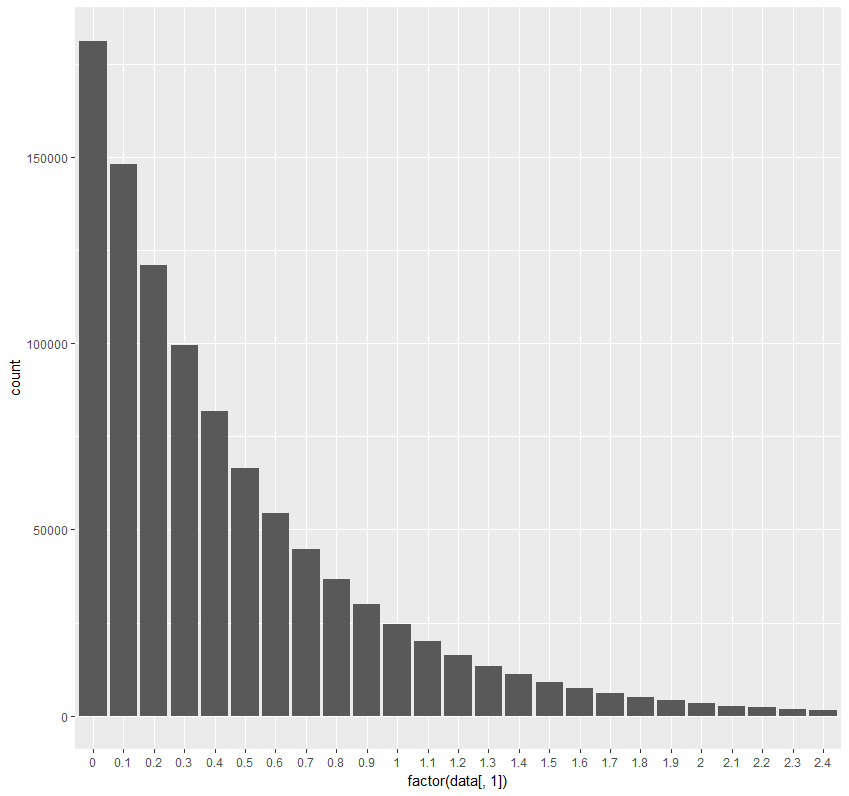
\includegraphics[scale=.6]{barplotexpo.png}
	\end{figure}
	This overall makes sense, as we will show below, 0 is the mode of the exponential distribution. This is confirmed as well by the barplot shown above.
	\item Find the Median and Mode of $X \sim $ Expo($\lambda $)
\end{enumerate}
\item Let X be Discrete Uniform on 1,2,3,4,5...n .
\begin{enumerate}
	\item  Use simulations in R to numerically estimate all medians and all modes of X for n = 1,2,3...10.
	\begin{verbatim}
	> #this is 3a
	> set.seed(433)
	> counter = 1
	> n=10
	> size = 1000
	> while(counter <= n)
	+ {
	+   binUnif(size,1,counter,1,1)
	+   counter = counter + 1
	+ }
	[1] "From 1 to 1"
	[1] 1
	1 
	1 
	[1] "From 1 to 2"
	[1] 1.505739
	1.0011387350969 
	1 
	[1] "From 1 to 3"
	[1] 2.025223
	1.00209179287776 
	1 
	[1] "From 1 to 4"
	[1] 2.502714
	1.00117637915537 
	1 
	[1] "From 1 to 5"
	[1] 2.957827
	1.00255306344479 
	1 
	[1] "From 1 to 6"
	[1] 3.368198
	1.00341863720678 
	1 
	[1] "From 1 to 7"
	[1] 4.004081
	1.0143808578141 
	1 
	[1] "From 1 to 8"
	[1] 4.470458
	1.00075664301403 
	1 
	[1] "From 1 to 9"
	[1] 5.058819
	1.0038467105478 
	1 
	[1] "From 1 to 10"
	[1] 5.422321
	1.01815693522803 
	1 
	\end{verbatim}
	\begin{figure}[H]
		\centering
		\caption{Mode across X demonstrated from Unif(1,1)}
		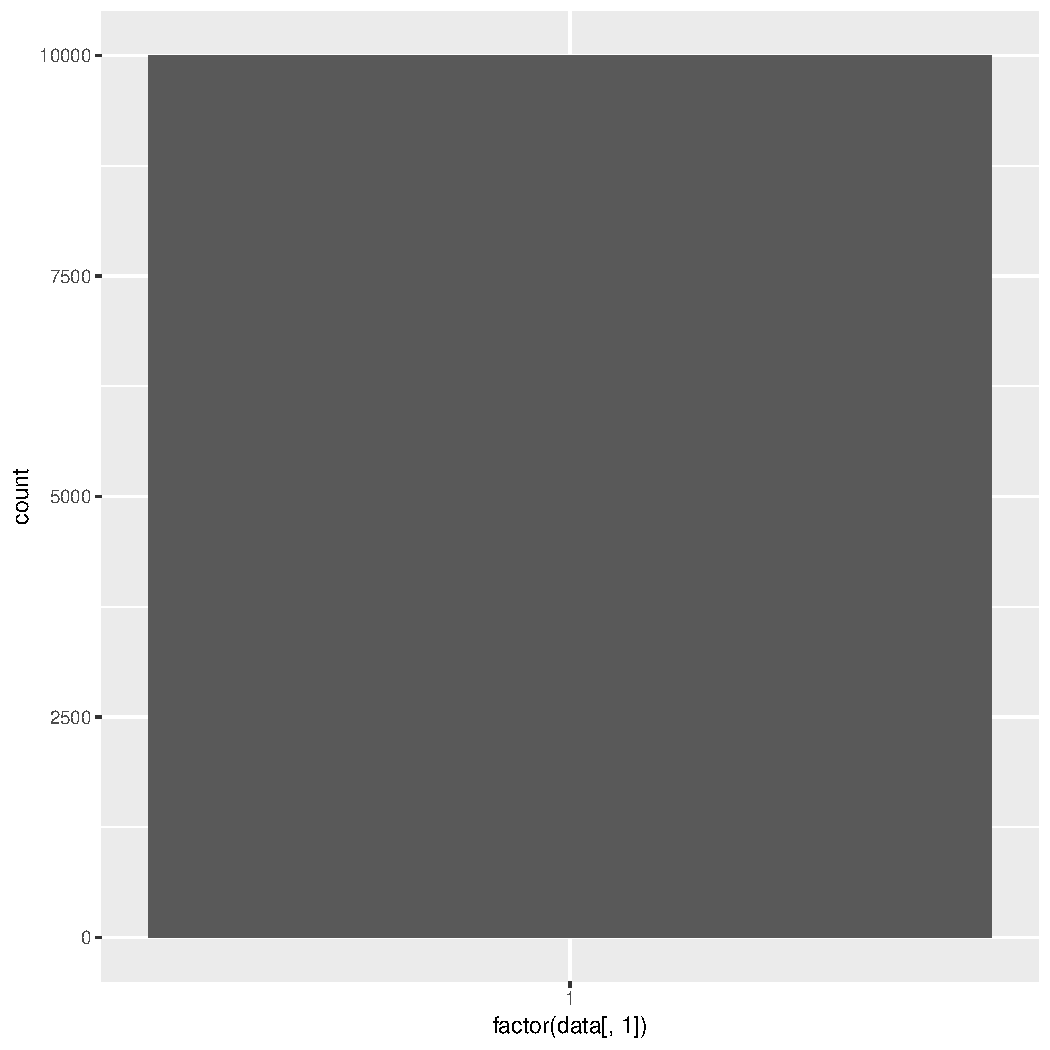
\includegraphics[scale=.4]{1graph.pdf}
	\end{figure}
	\begin{figure}[H]
		\centering
		\caption{Mode across X demonstrated from Unif(1,2)}
		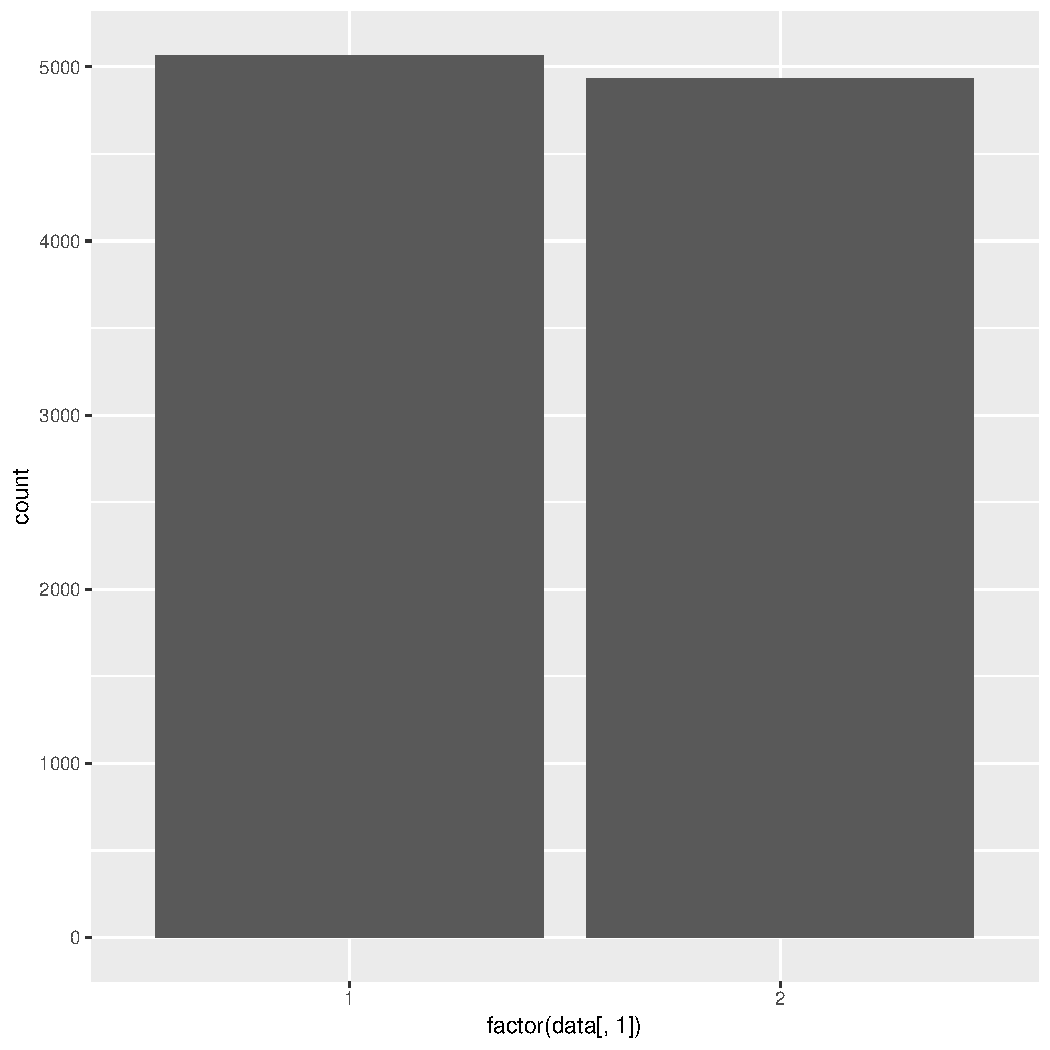
\includegraphics[scale=.4]{2graph.pdf}
	\end{figure}
	\begin{figure}[H]
		\centering
		\caption{Mode across X demonstrated from Unif(1,3)}
		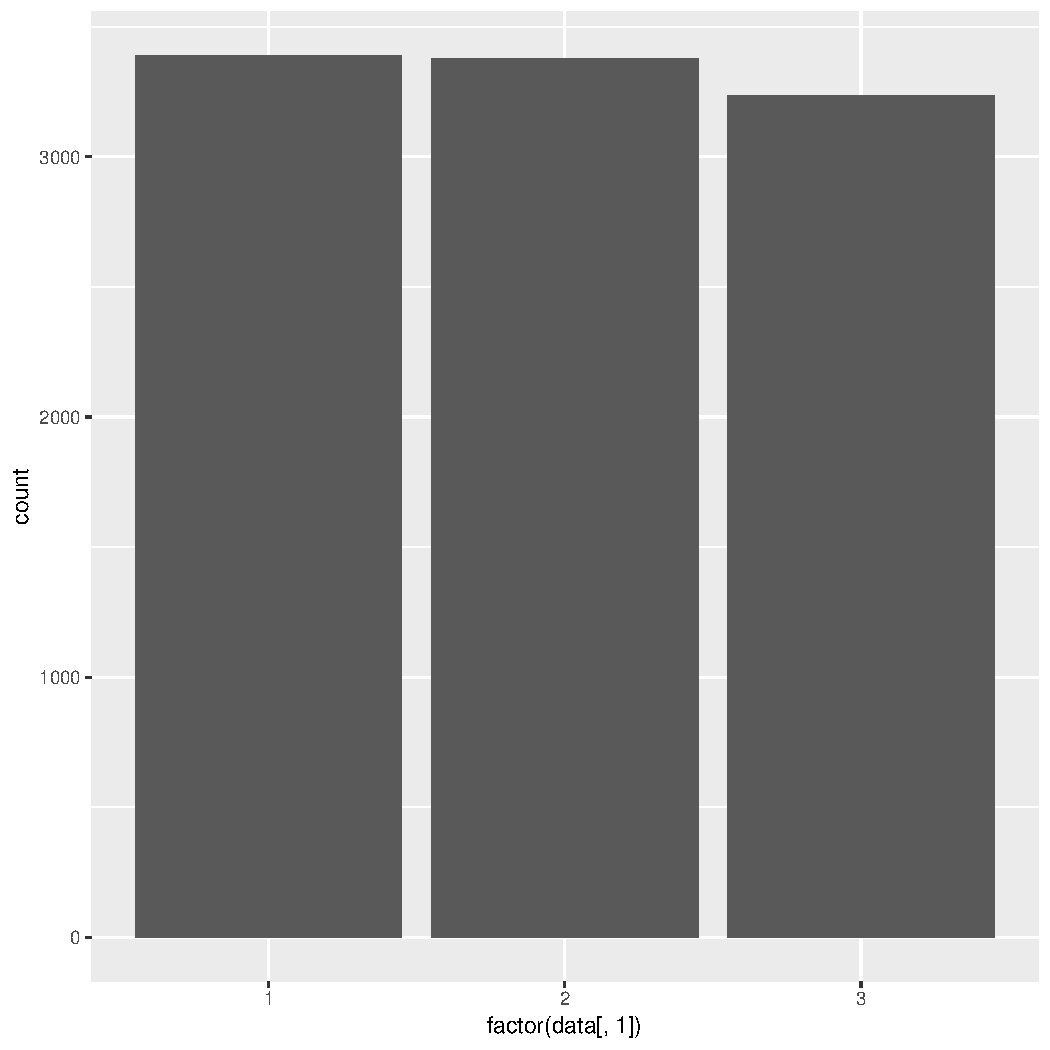
\includegraphics[scale=.4]{3graph.pdf}
	\end{figure}
	\begin{figure}[H]
		\centering
		\caption{Mode across X demonstrated from Unif(1,4)}
		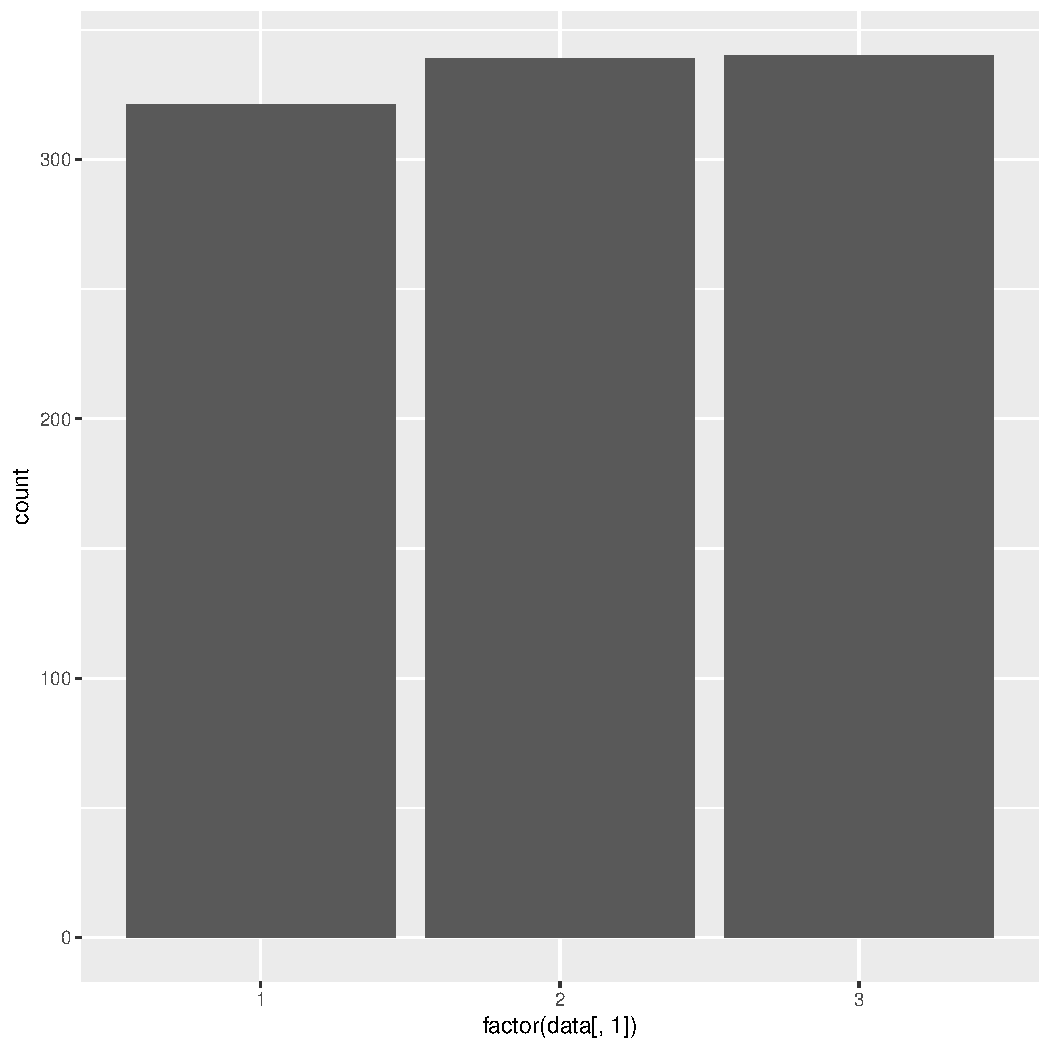
\includegraphics[scale=.4]{4graph.pdf}
	\end{figure}
	\begin{figure}[H]
		\centering
		\caption{Mode across X demonstrated from Unif(1,5)}
		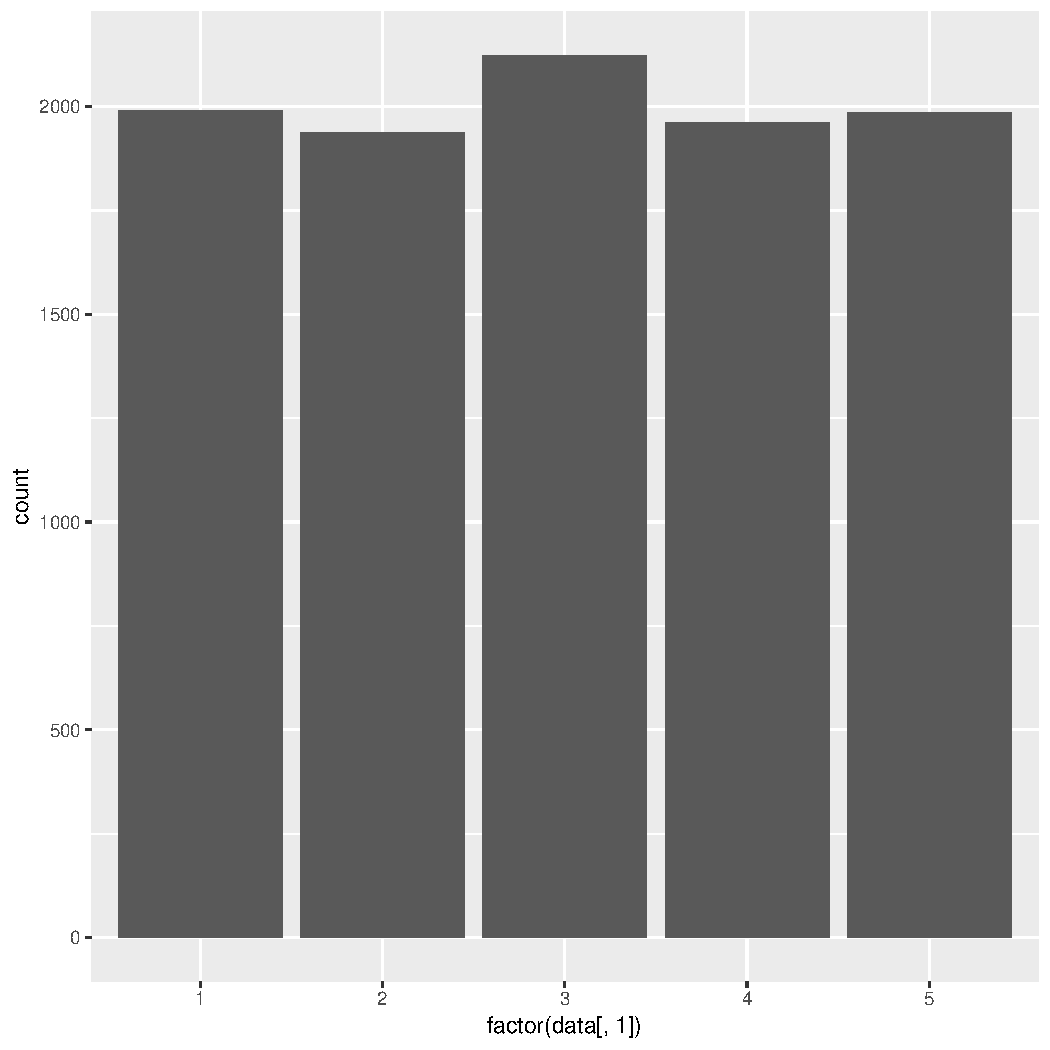
\includegraphics[scale=.4]{5graph.pdf}
	\end{figure}
	\begin{figure}[H]
		\centering
		\caption{Mode across X demonstrated from Unif(1,6)}
		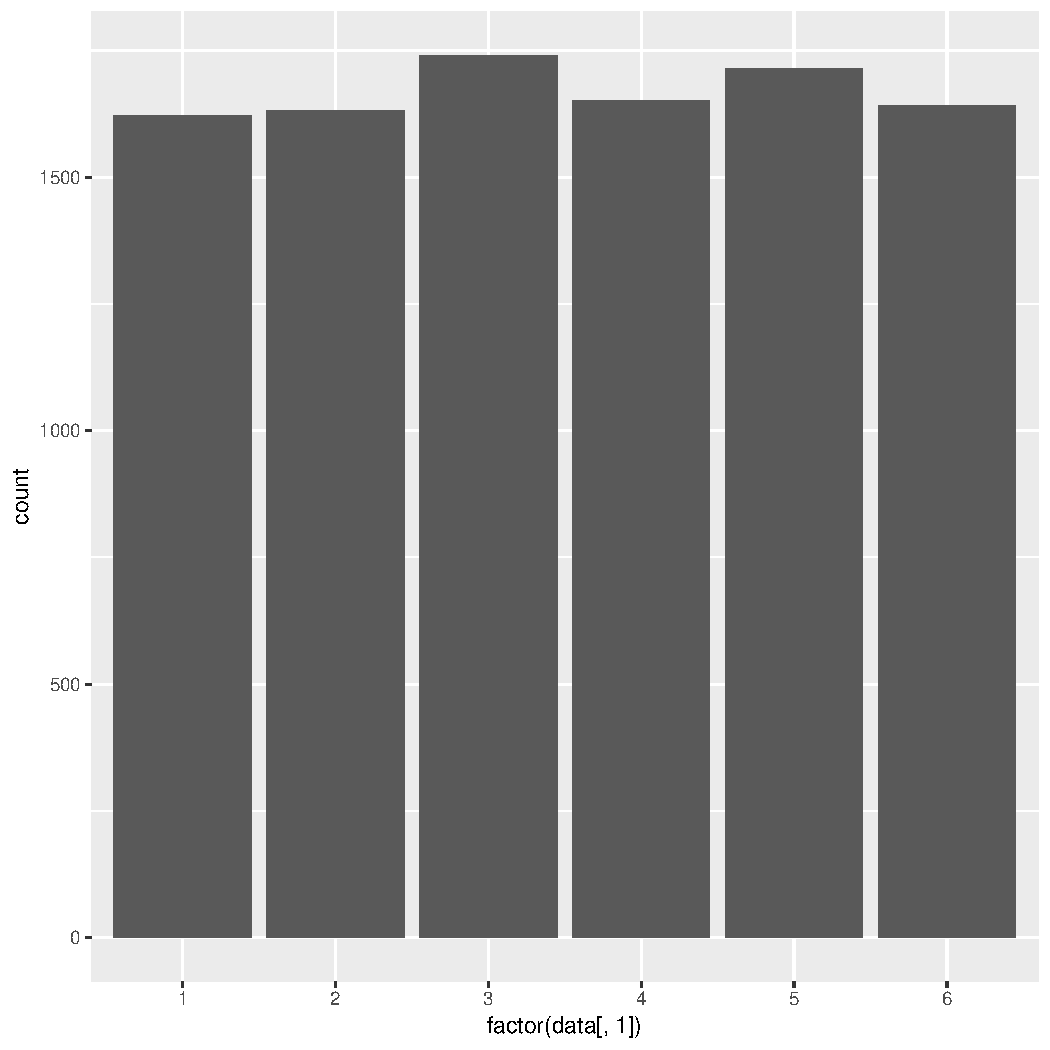
\includegraphics[scale=.4]{6graph.pdf}
	\end{figure}
	\begin{figure}[H]
		\centering
		\caption{Mode across X demonstrated from Unif(1,7)}
		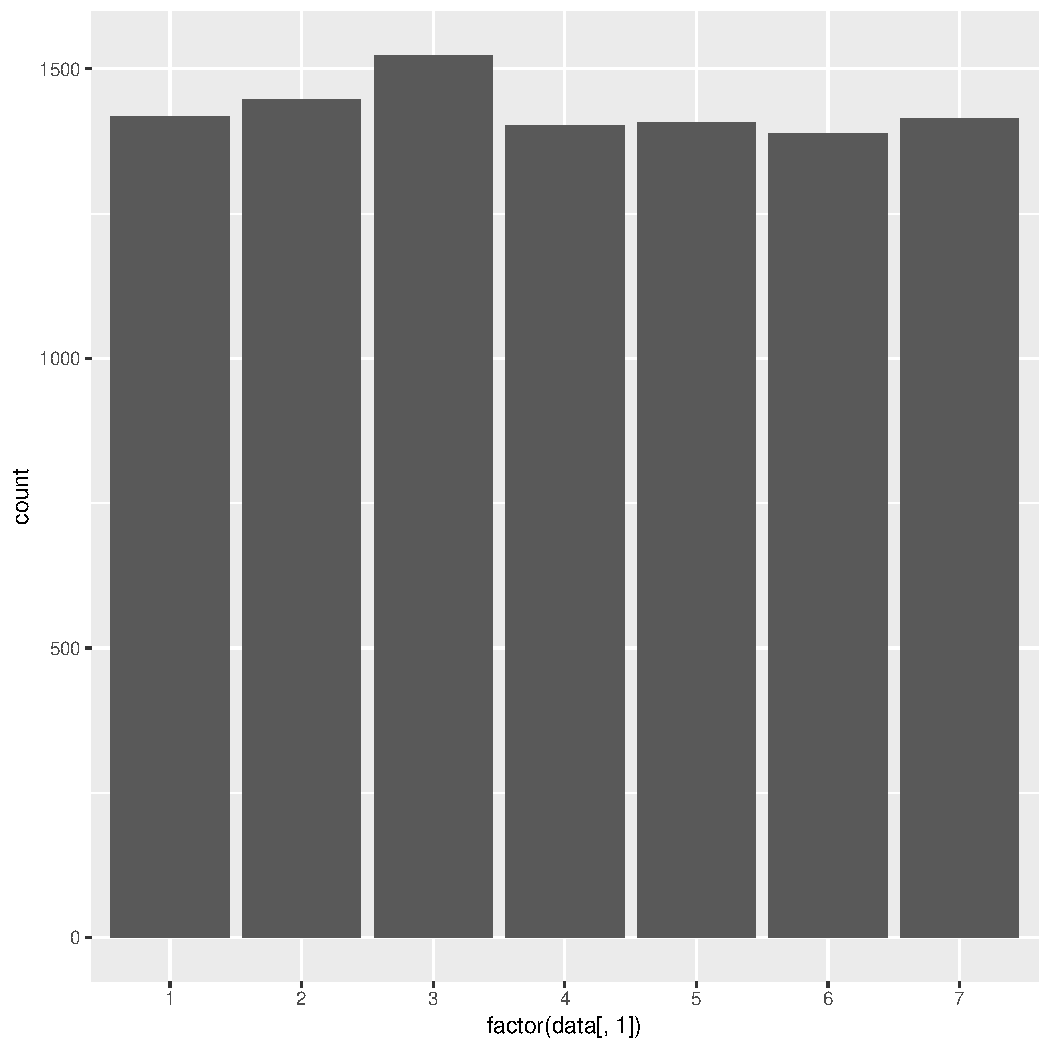
\includegraphics[scale=.4]{7graph.pdf}
	\end{figure}
	\begin{figure}[H]
		\centering
		\caption{Mode across X demonstrated from Unif(1,8)}
		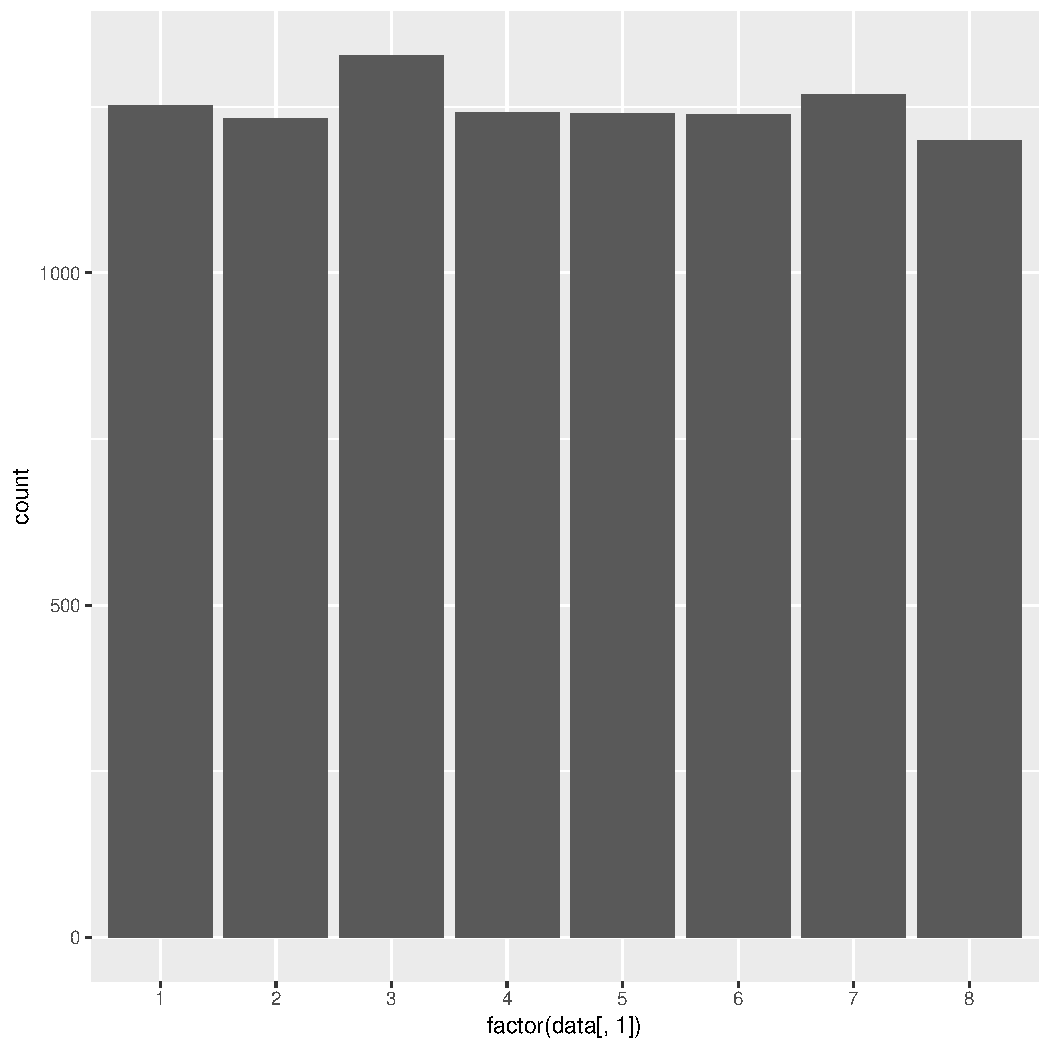
\includegraphics[scale=.4]{8graph.pdf}
	\end{figure}
	\begin{figure}[H]
		\centering
		\caption{Mode across X demonstrated from Unif(1,9)}
		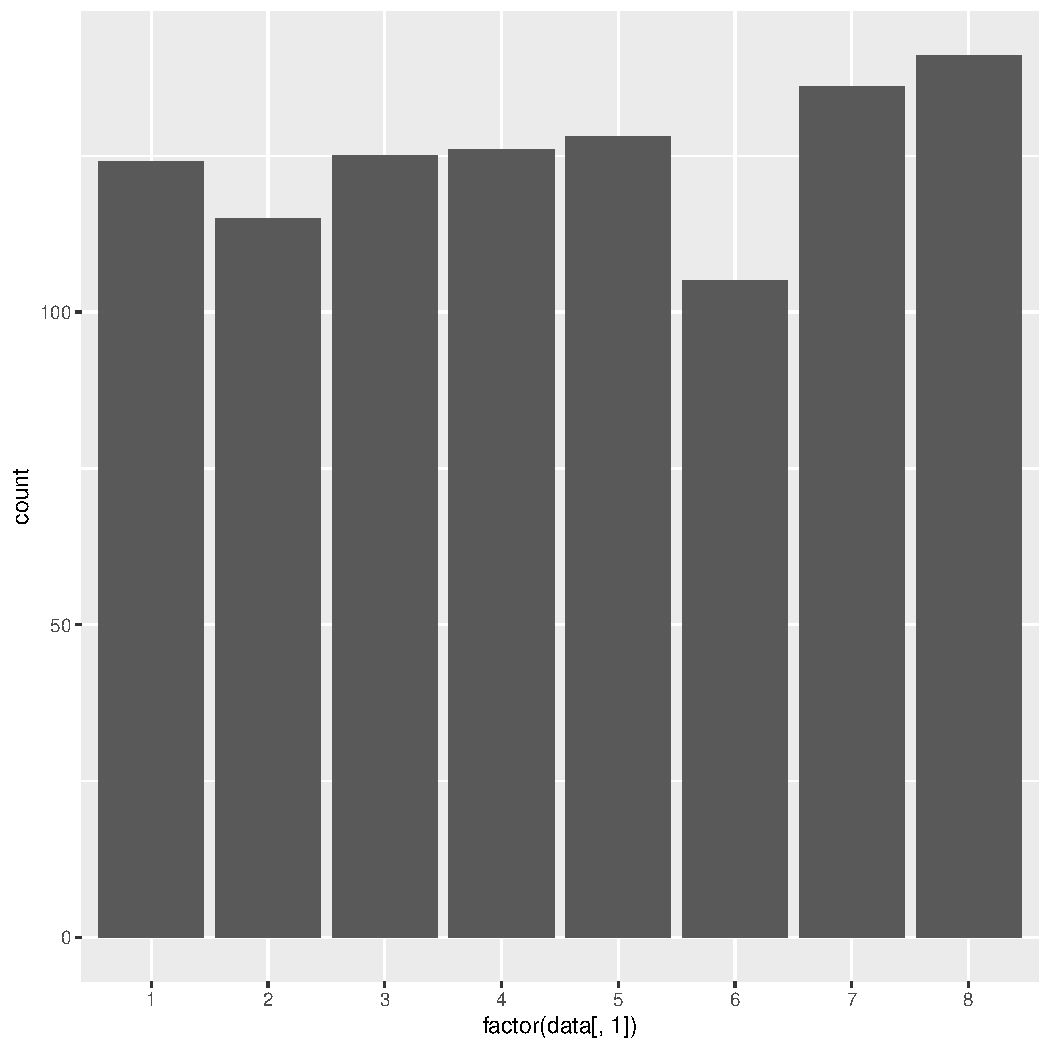
\includegraphics[scale=.4]{9graph.pdf}
	\end{figure}
	\begin{figure}[H]
		\centering
		\caption{Mode across X demonstrated from Unif(1,10)}
		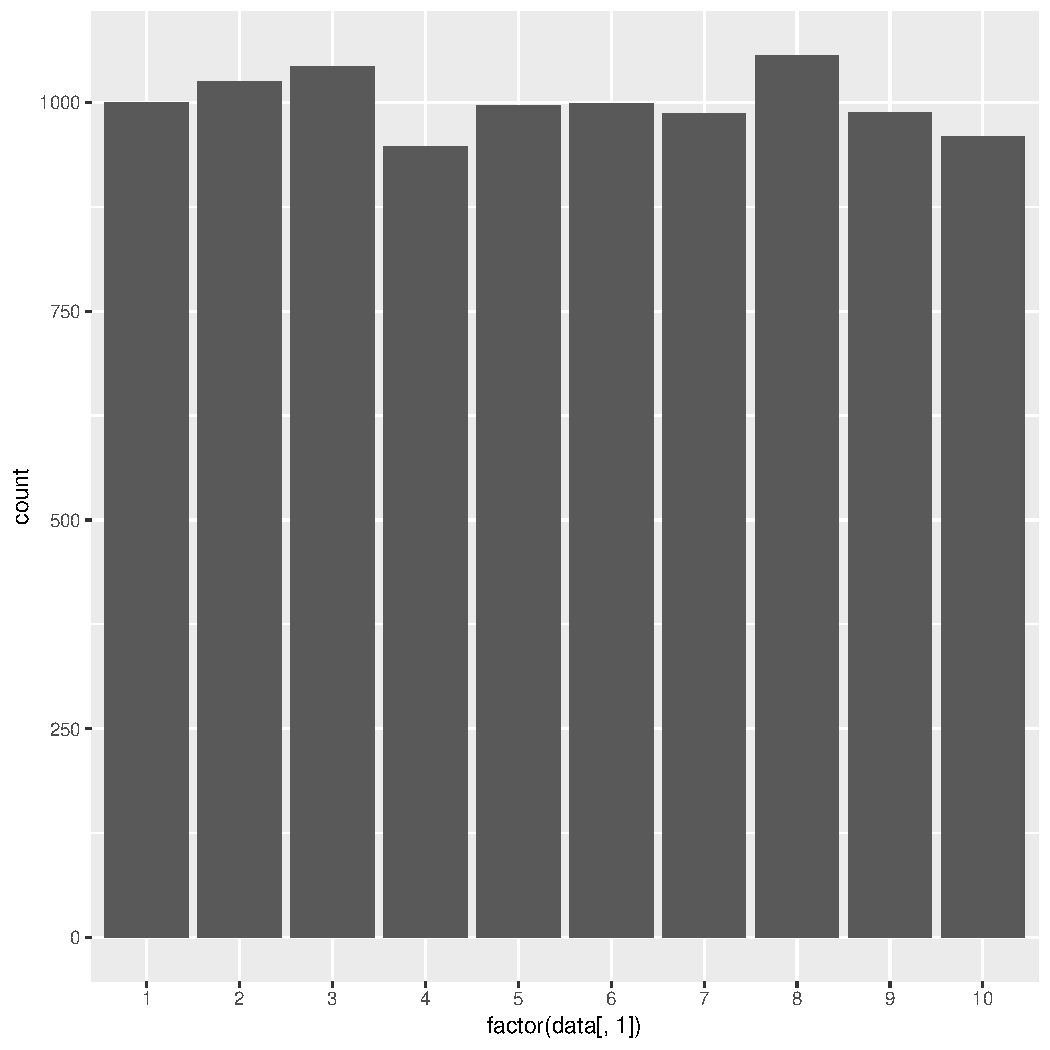
\includegraphics[scale=.4]{10graph.pdf}
	\end{figure}
	Again, we expect some variability here, but with large enough N we can understand that the mode of a discrete uniform distribution is over all discrete support of the RV
	\item Find All medians and modes of X\\
	Note the mode is trivial, as it is a similar case to 1.
	\begin{gather}
	\text{Want } P(X=c)\ge P(X=x)\forall x \in 1,2,...n\\
	=> \frac{1}{n-1+1} \ge \frac{1}{n-1+1}  \text{ by def of discrete Uniform}\\
	=> c=x \forall x \in 1,2,3,...n \text{ which is almost the same as 1}\\
	\text{Notable difference is that in the discrete case, c can only take discrete values}\\
	\text{Now the median}\\
	\text{Want } P(X\le x) \ge \frac{1}{2} \& P(X\ge x) \ge \frac{1}{2}\\
	P(X\le x) = \sum_{i=1}^{x}\frac{1}{n} = \frac{x}{n} \ge \frac{1}{2} => x \ge \frac{n}{2}\\
	\text{However, we can observe the patterns noted in the graphs below}\\
	\text{If n is odd, the previous conclusion is the only solution as }\\
	\text{if you go above or below } \frac{n}{2} \text{ you lose the probability @ } x = \frac{n}{2}\\
	\text{This is true as we have a jump exactly at }\frac{n}{2}\\
	\text{In the case n is even, you have some wiggle room}\\
	\text{There is no jump at }\frac{n}{2}\\
	\text{In fact, the next jump is at }\frac{n}{2}+1\\
	\text{This means we have medians from }[\frac{n}{2},\frac{n}{2}+1]\\
	\text{One last important factor to note, is that this result relies heavily on}\\
	\text{how we define the median and our environment}\\
	\text{In general we have}\\
	 Median(X) = 
	 \begin{cases}
	 \frac{n}{2} & n=\text{odd} \\
	 [\frac{n}{2},\frac{n}{2}+1] & n=\text{even}
	 \end{cases}
	\end{gather}
	\begin{figure}[H]
		\centering
		\caption{(n=5)Note the jumps taking place on the discrete values}
		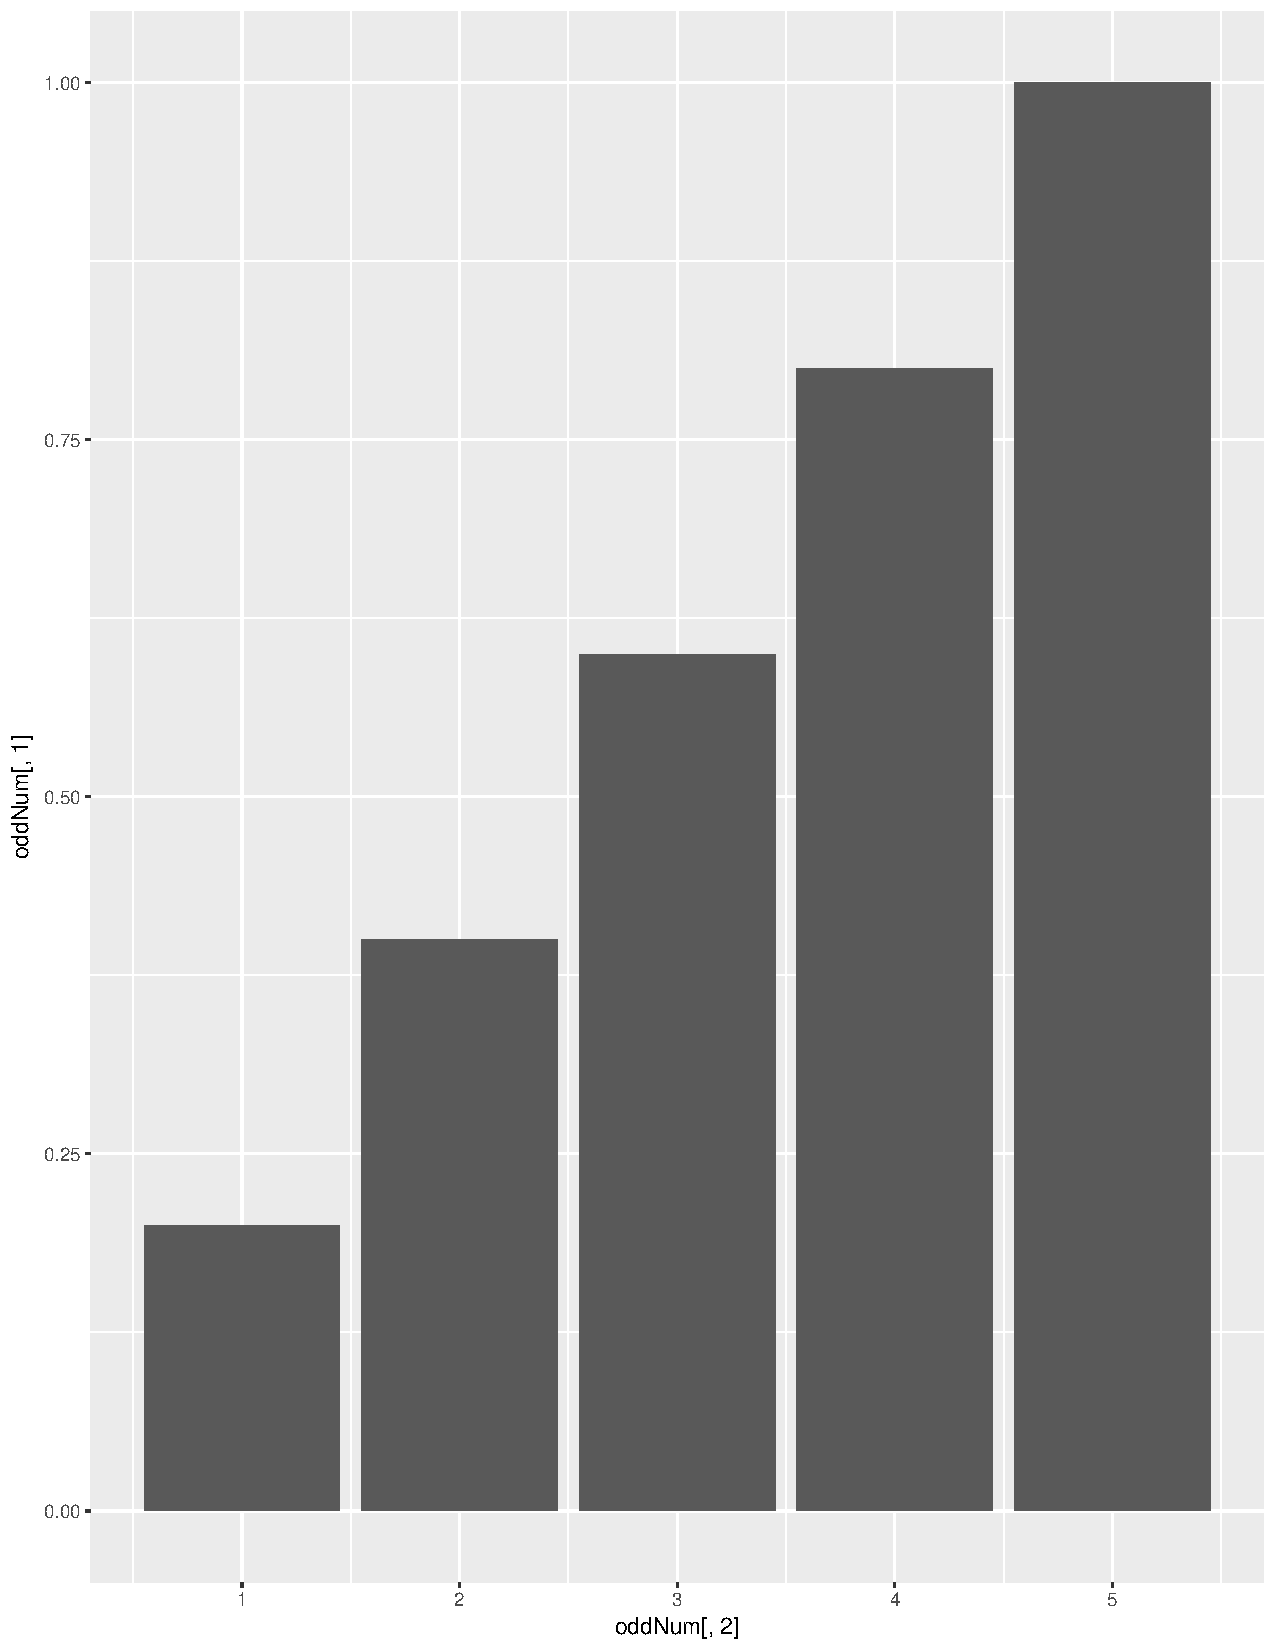
\includegraphics[scale=.4]{discreteOdd.pdf}
	\end{figure}
	\begin{figure}[H]
		\centering
		\caption{(n=6)These jump patterns hold for all discrete n}
		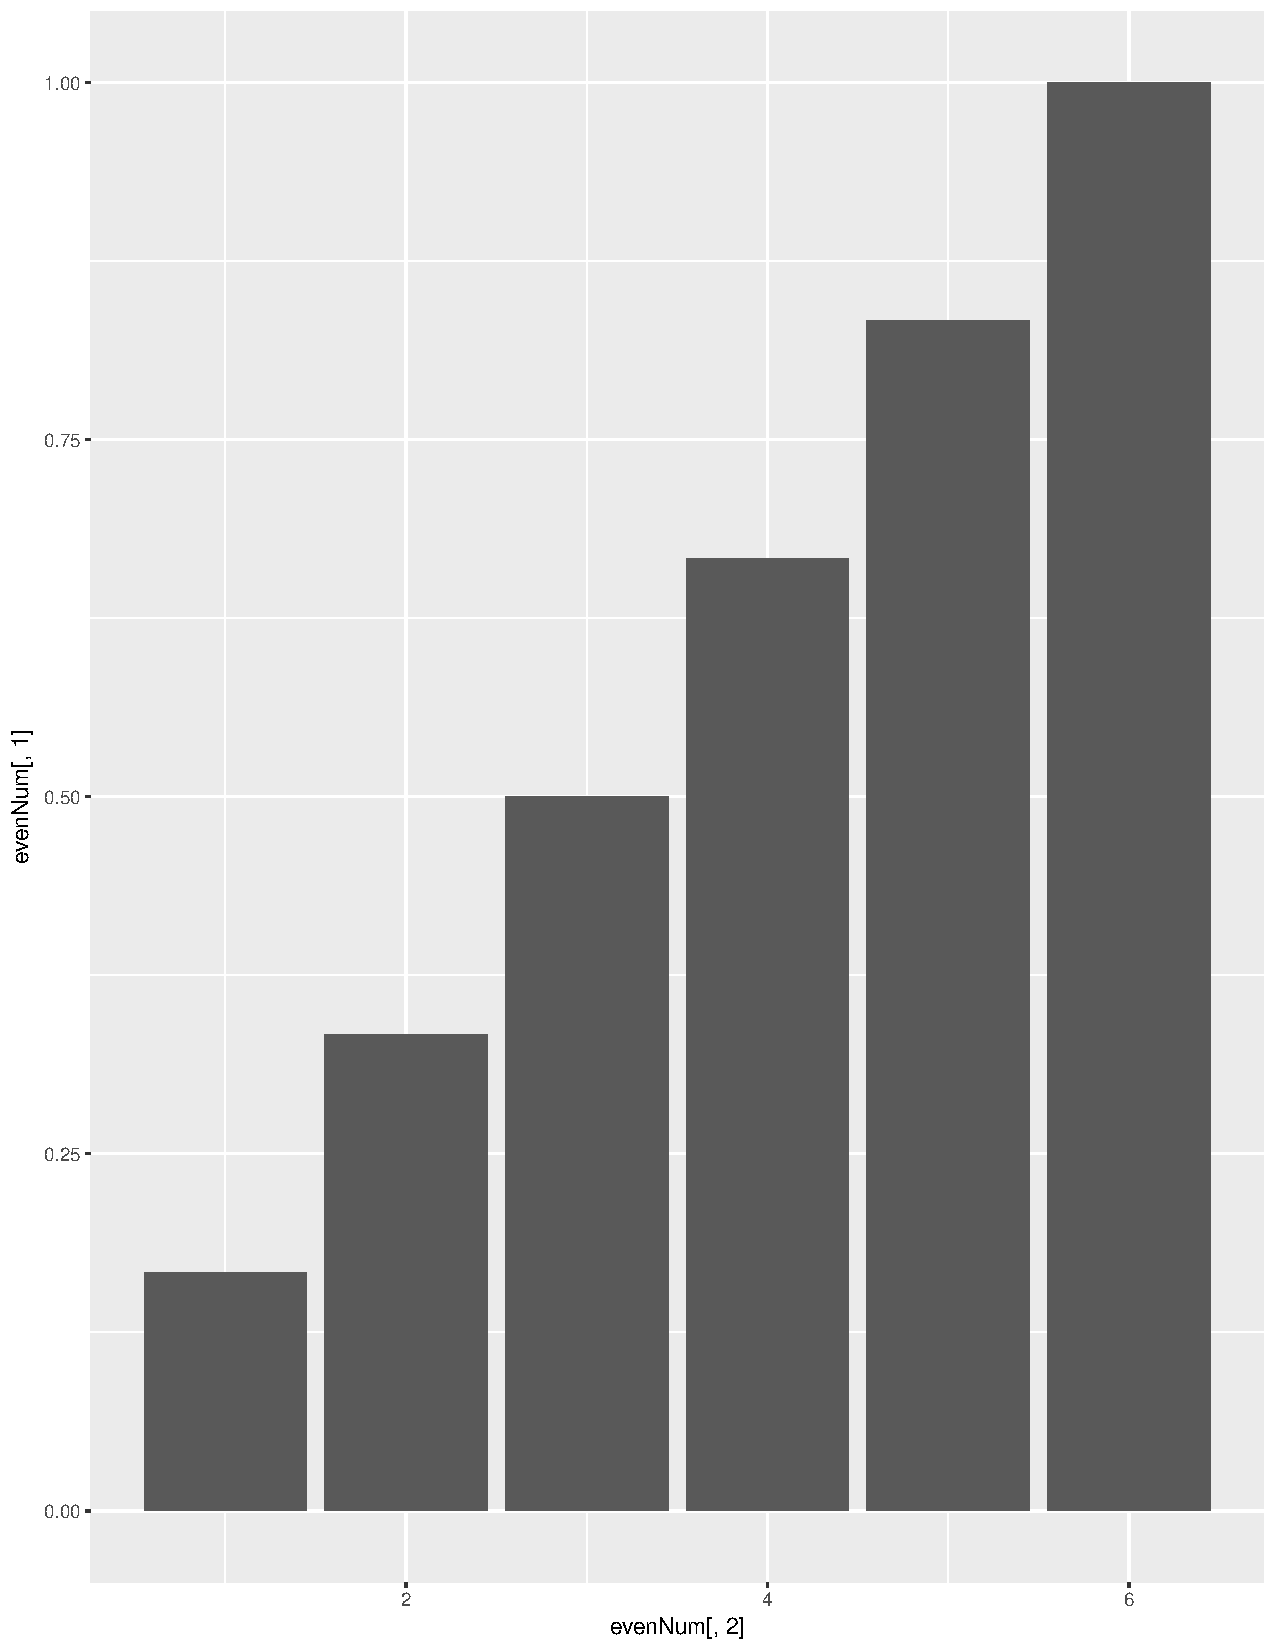
\includegraphics[scale=.4]{evenDisc.pdf}
	\end{figure}
\end{enumerate}
\item A distribution is called symmetric unimodal if it is symmetric (about some point) and has a unique mode.
For example, any Normal distribution is symmetric unimodal. Let X have a continuous symmetric unimodal
distribution for which the mean exists. Show that the mean, median, and mode of X are all equal.
\begin{gather}
	\text{First note that from our notes, we know the following}\\
	\text{1: The mean and median are on in the same by definition}\\
	\text{2: }f(x)=f(2\mu - x)\forall x \& P(X \ge X+\mu) = P(X\le X-\mu)\\
	\text{Where $\mu$ is the mean of our distribution, or central point}\\
	\text{All that is left to show is that the mode is equivalent to either our median or mean}\\
	\int_{-\infty}^{\mu - x} f(x)dx = \int_{\mu + x}^{\infty} f(x)dx = \int_{-\infty}^{\mu - x} f(2\mu - x)dx = \int_{\mu + x}^{\infty} f(2\mu - x)dx\\
	\int_{-\infty}^{\mu} f(x)dx = \frac{1}{2}= \int_{\mu}^{\infty} f(x)dx\\
	\text{By the defintion of the mode, we have some c } s.t. \, f(c) \ge f(x) \forall x\\
	\text{Lets proove via contradiction. If } c \ne \mu => c > \mu \text{ or } c<\mu\\
	=> f(c) = f(2\mu - c) \text{ with } c \ne 2\mu-c \text{ by our previous statement}\\
	=> \exists c_1 \, s.t. f(c_1)\ge f(x) \forall x \& c_2 \, s.t. f(c_2)\ge f(x) \forall x \text{ with } c_1 \ne c_2\\
	\text{This is a contradiction! as now we have two unique modes}\\
	\text{ which violates the property of a unimodal distribution} \square
\end{gather}
\item Let $W = X^2 + Y^2$, with X, Y i.i.d. N(0, 1). You can assume you know that the MGF of $X^2$ is $(1 - 2t)^{\frac{-1}{2}}$ for $t < \frac{1}{2}.$ 
Find the MGF of W.
\begin{gather}
	\text{We know for independent X, Y random variables that } M_{X+Y}(t)=M_X(t)*M_Y(t) \\
	\text{We know that }M_{X^2}(t)=M_{Y^2}(t) \text{ and lets rewrite }X'=X^2 and Y' = Y^2\\
	\text{since } X' \& Y' \text{ independet } => M_{X'+Y'}=M_{X'}*M_{Y'}=M_{X^2}*M_{Y^2}=((1 - 2t)^{\frac{-1}{2}})^2 =\frac{1}{1-2t}
\end{gather}
\item Let $X \sim Expo(\lambda)$. You can assume you know that $\lambda X \sim$ Expo(1), and that the nth moment of an Expo(1) random variable is n!. Find the skewness of X.
\begin{gather}
	\text{Def of Skewness(X): } E[(\frac{X-\mu}{\sigma})^3]\\
	= E[(\frac{X-E[X]}{\sqrt{\Var(X)}})^3]=E[(\frac{X-\frac{1}{\lambda}}{\sqrt{\frac{1}{\lambda^2}}})^3] = E[(\lambda(X-\frac{1}{\lambda}))^3]= E[(\lambda X-1)^3] \\
	= E[(\lambda X)^3-3(\lambda X)^2 + 3(\lambda X) - 1] = E[(\lambda X)^3] - 3E[(\lambda X)^2] + 3E[(\lambda X)] - 1\\
	\text{With }E[(\lambda X)^3] = 3!, E[(\lambda X)^2] = 2!, E[(\lambda X)]=1! \text{ from problem statement}\\
	=> E[(\frac{X-E[X]}{\sqrt{\Var(X)}})^3] = 3! - 3*2 + 3*1 - 1 = 2
\end{gather}
\item Let $X_1,...X_n$ be i.i.d. with mean $\mu$, variance $\sigma^2$, and MGF M. Let \\
 $\bar{X_n}=\frac{1}{n}\sum_{i=1}^{n} X_i$ 
 and
 $Z_n = \sqrt{n}\frac{\bar{X_n}-\mu}{\sigma}$
\begin{enumerate}
	\item Show that $Z_n$ has mean 0 and variance 1
	\begin{gather}
		E[\bar{X_n}]=E[\frac{1}{n}\sum_{i=1}^{n} X_i] = \frac{1}{n}\sum_{i=1}^{n} E[X_i] =  \frac{1}{n} * n\mu =\mu\\
		=> E[Z_n] = E[\sqrt{n}\frac{\bar{X_n}-\mu}{\sigma}] = \sqrt{n}\frac{E[\bar{X_n}]-\mu}{\sigma} = 0\\
		\Var(\bar{X_n}) = \Var(\frac{1}{n}\sum_{i=1}^{n} X_i) = \frac{1}{n^2}\sum_{i=1}^{n} \Var(X_i) = \frac{1}{n^2} n\sigma^2=\frac{\sigma^2}{n}\\
		=> \Var[Z_n]=\Var(\sqrt{n}\frac{\bar{X_n}-\mu}{\sigma}) = \frac{n}{\sigma^2}\Var(\bar{X_n}-\mu) = \frac{n}{\sigma^2}\Var(\bar{X_n})= \frac{n}{\sigma^2}\frac{\sigma^2}{n}=1
	\end{gather}
	\item Find the MGF of $Z_n$ in terms of M, the MGF of each $X_i$
	\begin{gather}
		MGF_{Z_n}(t)=e^{Z_nt} = e^{\sqrt{n}\frac{\bar{X_n}-\mu}{\sigma}t} =  e^{t\sqrt{n}\frac{\bar{X_n}}{\sigma} -t\sqrt{n}\frac{\mu}{\sigma}} = e^{\frac{t\sqrt{n}}{n\sigma}\sum_{i=1}^{n} X_i}e^{-t\sqrt{n}\frac{\mu}{\sigma}}\\
		\text{Note MGF}(X_i) = M = e^tX \text{ where t is any real}\\
		\text{Now let }\frac{t\sqrt{n}}{n\sigma} = t' \\
		=> MGF_{Z_n} = e^{t'\sum_{i=1}^{n} X_i}e^{-t\sqrt{n}\frac{\mu}{\sigma}} =  e^{t'X_1+t'X_2...t'X_n}e^{-t\sqrt{n}\frac{\mu}{\sigma}}= \prod_{i=1}^{n}Me^{-t\sqrt{n}\frac{\mu}{\sigma}} = M^ne^{-t\sqrt{n}\frac{\mu}{\sigma}}
	\end{gather}
\end{enumerate}
\end{enumerate}

\end{document}
